\chapter{Heterogeneity in the MAX phases}
\label{chap:hetero_max_phases}

\graphicspath{{hetero_max_phases/Figs/}}


As  discussed in \autoref{sec:ductility_criteria}, the MAX phases are predicted to be brittle by a wide range of ductility criteria but they are in fact observed to be damage tolerant and to flow easily in the basal plane \cite{Barsoum1999}.
Predictions of the Peierls stress made using the methods described in \autoref{sec:dislocations} have been made previously \cite{Music2007ductility,Gouriet2015}. However these have had limited success, producing over-estimates, for example \citet{Gouriet2015} reported the Peierls stress to be at least \SI{611}{\mega\pascal} which is similar to  that estimated for titanium carbide and other very hard brittle materials in which slip is limited at room temperature by the Peierls mechanism \cite{Chang1966,Clegg2006,Kamimura2011,Yadav2014}. Given that flow stresses in the region of a few tens of \si{\mega\pascal} have been observed at room temperature \cite{Humphrey2012,Barsoum1999}, which is more comparable with FCC metals than FCC carbides, it is reasonable to expect the Peierls stress of MAX phases to be lower than that of TiC.

The poor performance of Peierls models for MAX phases, and potentially for other complex phases, might be due to the treatment of the MAX phase unit cell as elastically homogeneous. This is surprising because many studies have discussed the heterogeneity of the bonding and electron structure. One recent review was written by \citet{Magnuson2017}, and discusses the complex and mixed nature of the bonding varying across the different atomic sites: more metallic in the MA layers, more covalent in the MX layers, and charge transfer contributing an ionic component to the bonding. 

The bonding is associated with many of the properties of the MAX phases, for example high melting point, high specific stiffness, electrical and thermal conductivity, and a near zero Seebeck coefficient to name a few \cite{Yoo2000,Sun2011,Magnuson2017}. However the clear and strong heterogeneity of the unit cell has largely been neglected when considering the mechanical properties of the MAX phases, the only consideration of the atomic environments  being the choice of plane at which the generalised stacking fault energy was calculated \cite{Music2007ductility}.


\section{Chemical heterogeneity}

Measuring single crystal elastic constants for the MAX phases is extremely difficult due to the difficulty of growing single crystals and experimentally determining the stiffness of sub-unit cell regions of the crystal presents an even greater challenge. Instead density functional theory can be employed. DFT has been widely used to calculate single crystal elastic constants of a large variety of materials and is considered reliable and reproducible \cite{Lejaeghere2016}. 



If the MAX phases are elastically heterogeneous, there is the question of what might be the expected properties and how these might vary within the MAX phase unit cell. A simple way of characterising the chemical heterogeneity is the electronegativity, $\chi$, of regions within the unit cell. For both the M--X and M--A regions, an average electronegativity is easily calculated, as once sharing of atoms between the regions is accounted for, there are equal numbers of M and A atoms in the M--A region and similarly equal numbers of M and X atoms in the M--X region. The difference in electronegativity between the two regions is therefore defined by
\begin{equation}
\Delta \chi = \frac{\chi_{\text{X}} - \chi_{\text{A}}}{2}\label{eqn:MAX_electronegativity_diff}
\end{equation}
since the M atoms contribute to both regions. 

There are a variety of measures of electronegativity, but perhaps the most fundamental and transferable is the Mulliken scale \cite{Mulliken1934}, which takes the electronegativity of a species to be the average of the ionization energy, the energy change upon removing an electron, and the electron affinity, the energy change upon adding an electron. This scale is more fundamental than others because it is calculated from the fundamental properties of atoms, as opposed to more ``relative'' scales that are calculated from enthalpies of formation and covalent radii and so on \cite{huheey1983ch3_electronegativity}.

Since the elements that take the X site, carbon and nitrogen, are generally more electronegative than those that take the A site, elements like aluminium and silicon, it is expected that electron transfer into the M--X region from the M--A \cite{Sun2011}. Such a transfer would be expected to increase the strength of the bonding in the M--X layer and reduce it in the M--A, with a corresponding change in the moduli of the two regions.


\section{Density functional theory calculations}
\label{sec:DFT_method}



Measuring single crystal elastic constants for the MAX phases is challenging due to the difficulty of growing single crystals and experimentally determining the stiffness of sub-unit cell regions of the crystal presents an even greater challenge. Instead density functional theory (DFT) can be employed. DFT has been widely used to calculate single crystal elastic constants of a large variety of materials and is considered reliable and reproducible \cite{Lejaeghere2016}. 

%%% Better check I've referenced this correctly and that I understand it enough
The density functional theory calculations were performed with the SIESTA package \cite{soler2002}, a pseudopotential-based LCAO package using semicore pseudopotentials with partial core corrections in the Perdew-Burke-Ernzhof (PBE) formulation generated and tested by the ATOM implementation \cite{soler2002} of the Troullier-Martins procedure \cite{Troullier1991,Troullier1991a} as described in the software documentation \cite{ATOM_manual}. A double-$\zeta$ polarised basis set including the semicore states was used, the cutoff radii of which were optimised with a variational simplex method.

The starting point for the calculations presented here were a series of optimised unit cells for a range of MAX phases produced by a procedure developed by Philip Howie. A optimisation approach to generating suitable pseudopotentials was taken using ATOM \cite{ATOM_manual}; pseudopotentials with a range of cut off radii were tested against all-electron calculations of the atomic ground state and a number of excited states and the cut off radius is improved until the best (i.e. closest to all-electron) pseudopotential is identified. 

Initially some simulation parameters have to be optimised: the k-grid size and the mesh cut off. Suitable values are chosen to provide sufficient accuracy and ensure the energy converges \cite{SIESTA_manual}.

Once pseudopotentials and the simulation parameters have been generated the lattice parameters are optimised. The literature values are used as the starting point but the calculated equilibrium lattice parameter is typically \SIrange{1}{2}{\percent} bigger that the experimental value when using the generalised gradient approximation \cite{Staroverov2004,Wu2006,Staroverov2008erratum}. Initially the lattice parameter ratio, $c/a$, is kept fixed and the lattice parameter $a$ is varied to reduce the hydrostatic pressure to zero.

The basis set was optimised with this roughly equilibrated unit cell. Most of the variables are taken to be suggested values  from examples provided by the authors of SIESTA \cite{SIESTA_manual}. The problem is variational (i.e. a lower energy means a better basis set) so the basis set is optimised by the simplex optimisation method, also known as the Nelder-Mead method \citep{Nelder1965}. With an accurate basis set the lattice parameters are now optimised to find the true equilibrium point, relaxing both $a$ and $c$ to reduce the stresses to zero (or equivalently finding the minimum energy). Many of the atomic positions are fixed by symmetry, but those parameters that are free to vary without breaking the structure's symmetry are relaxed. These are the heights in the $c$-axis of some of the atoms as shown in \autoref{fig:MAX_unit_cells}.


A comparison of the lattice parameters generated by DFT with Howie's method is shown in \autoref{fig:unit_cells_DFT_vs_literature} and the data are summarised in \autoref{tab:MAX_DFT_unit_cell_results}. The agreement is good as expected, particularly in the lattice geometry, $c/a$. The better agreement in $c/a$ than in the lattice parameters themselves is because the errors in the lattice parameters are correlated, in that both $a$ and $c$ are overestimated as expected with the PBE formulation \cite{Staroverov2004,Staroverov2008erratum}. These equilibrated unit cells were used as the basis for further investigation of MAX phase behaviour.

\begin{figure}
\begin{subfigure}{0.4\textwidth}

\centering
\captionsetup{width=\textwidth}
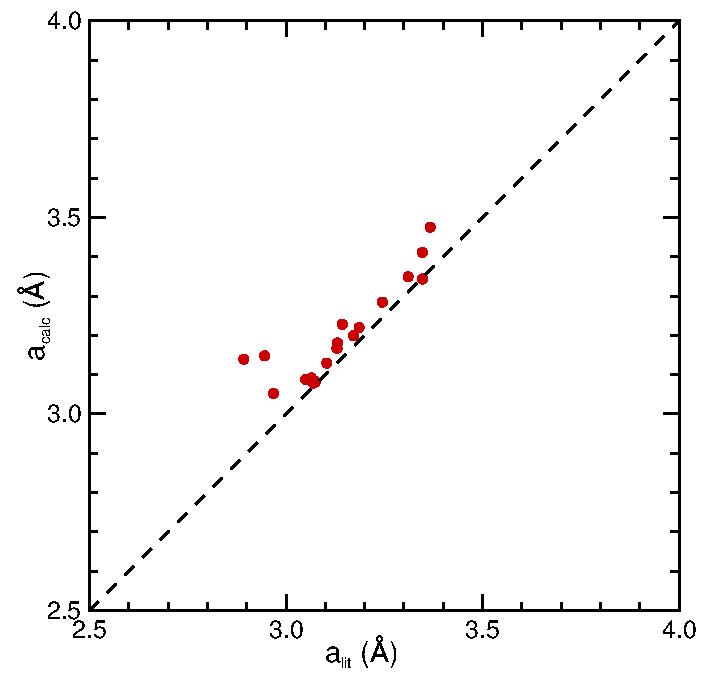
\includegraphics[width=\textwidth]{a_calc_vs_a_lit}
\caption[Calculated lattice parameters compared with literature values]{A comparison between the lattice parameter, $a$, calculated here with literature values.\label{fig:latt_params_DFT_vs_lit}}

\end{subfigure}
~
\begin{subfigure}{0.4\textwidth}
\centering
\captionsetup{width=\textwidth}
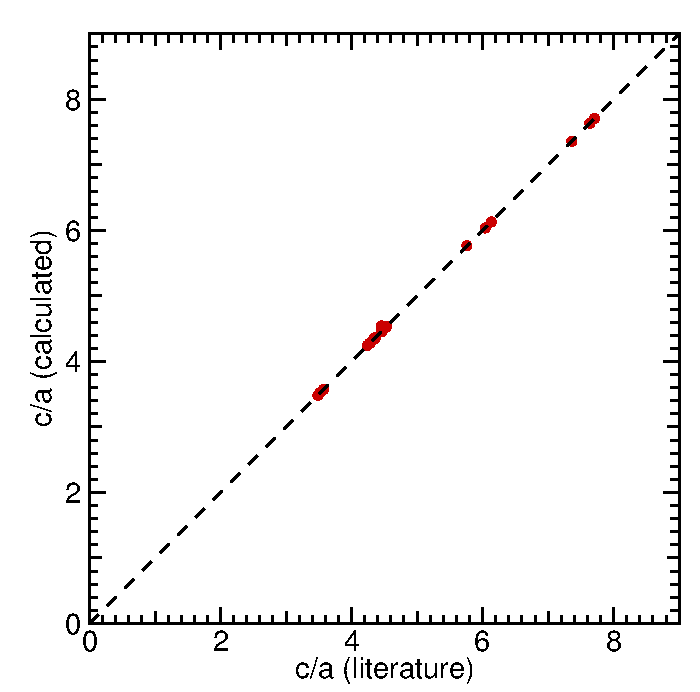
\includegraphics[width=\textwidth]{c-a_calc_vs_lit}
\caption{A comparison between the calculated lattice parameter ratio, $c/a$, with literature values.\label{fig:c_a_ratio_DFT_vs_lit}}
\end{subfigure}

\caption[A comparison of the unit cells calculated by DFT with the literature.]{A comparison of the unit cells calculated by DFT with those reported in the literature. There is reasonable agreement between the lattice parameters $a$ calculated here and found experimentally in the literature. The lattice geometry, $c/a$, is in excellent agreement with reported values.\label{fig:unit_cells_DFT_vs_literature}}
\end{figure}



\begin{sidewaystable}
\begin{tabular}{|l|c|c|c|c|c|c|c|c|c|c|c|c|c|c|}
\hline
Phase &       $a$ &     $a_{\text{lit}}$ &     $c/a$ & $c/a_{\text{lit}}$ &       $z_1$ &    $z_{1,\text{lit}}$ &       $z_2$ &   $z_{2,\text{lit}}$ &      $z_3$ &    $z_{3,\text{lit}}$ &       $d/b$ &     $z_{\text{M--A}}$ &      $d_{\text{M--A}}$ \\
\hline
   \ce{Nb2AlC}\rule[3ex]{0pt}{0pt} &  3.1297 &  3.1035 &  4.5215 &  4.5213 &  0.0898 &  0.0880 &       - &       - &       - &       - &  0.7243 &  0.1602 &  2.2479 \\
   \ce{Nb2GaC}                     &  3.1806 &  3.1310 &  4.3322 &  4.3325 &  0.0887 &  0.0880 &       - &       - &       - &       - &  0.6988 &  0.1613 &  2.1880 \\
   \ce{Nb2InC}                     &  3.1987 &  3.1720 &  4.5303 &  4.5303 &  0.0827 &  0.0860 &       - &       - &       - &       - &  0.7579 &  0.1673 &  2.4041 \\
    \ce{Nb2SC}                     &  3.3484 &  3.3100 &  3.4862 &  3.4864 &  0.0944 &  0.0990 &       - &       - &       - &       - &  0.5425 &  0.1556 &  1.7956 \\
   \ce{Nb2SnC}                     &  3.2844 &  3.2450 &  4.2441 &  4.2435 &  0.0833 &  0.0850 &       - &       - &       - &       - &  0.7074 &  0.1667 &  2.2954 \\
   \ce{Ti2AlC}                     &  3.0517 &  2.9680 &  4.5422 &  4.4554 &  0.0844 &  0.0882 &       - &       - &       - &       - &  0.7378 &  0.1656 &  2.1898 \\
   \ce{Ti2GaC}                     &  3.0914 &  3.0640 &  4.3431 &  4.3424 &  0.0855 &  0.0880 &       - &       - &       - &       - &  0.7143 &  0.1645 &  2.1887 \\
   \ce{Ti2InC}                     &  3.1481 &  2.9450 &  4.4905 &  4.4852 &  0.0790 &  0.0829 &       - &       - &       - &       - &  0.7670 &  0.1710 &  2.2587 \\
    \ce{Ti2SC}                     &  3.2279 &  3.1432 &  3.5172 &  3.5158 &  0.0977 &  0.0998 &       - &       - &       - &       - &  0.5355 &  0.1523 &  1.6830 \\
   \ce{Ti2SnC}                     &  3.2196 &  3.1860 &  4.2786 &  4.2781 &  0.0807 &  0.0790 &       - &       - &       - &       - &  0.7243 &  0.1693 &  2.3076 \\
   \ce{Zr2InC}                     &  3.3434 &  3.3470 &  4.4541 &  4.4547 &  0.0874 &  0.0860 &       - &       - &       - &       - &  0.7243 &  0.1626 &  2.4243 \\
    \ce{Zr2SC}                     &  3.4755 &  3.3663 &  3.5711 &  3.5714 &  0.0998 &  0.1013 &       - &       - &       - &       - &  0.5364 &  0.1502 &  1.8058 \\
   \ce{Zr2SnC}                     &  3.4110 &  3.3470 &  4.3590 &  4.3591 &  0.0854 &  0.0860 &       - &       - &       - &       - &  0.7175 &  0.1646 &  2.4015 \\
  \ce{Ti3AlC2}                     &  3.0831 &  3.0730 &  6.0390 &  6.0387 &  0.0710 &  0.0691 &  0.1305 &  0.1276 &       - &       - &  0.7216 &  0.1224 &  2.2714 \\
  \ce{Ti3SiC2}                     &  3.0820 &  3.0747 &  5.7642 &  5.7620 &  0.0727 &  0.0722 &  0.1355 &  0.1353 &       - &       - &  0.6600 &  0.1147 &  2.0321 \\
  \ce{Nb4AlC3}                     &  3.1674 &  3.1296 &  7.7081 &  7.7073 &  0.0549 &  0.0552 &  0.1088 &  0.1086 &  0.1575 &  0.1574 &  0.7130 &  0.0926 &  2.2345 \\
  \ce{Ti4GaC3}                     &  3.0781 &  3.0690 &  7.6371 &  7.6377 &  0.0516 &  0.0558 &  0.1091 &  0.1068 &  0.1549 &  0.1564 &  0.7263 &  0.0936 &  2.1940 \\
 \ce{Ti4SiC3}\rule[-1ex]{0pt}{0pt} &  3.0878 &  3.0500 &  7.3627 &  7.3614 &  0.0535 &  0.0532 &  0.1120 &  0.1118 &  0.1603 &  0.1599 &  0.6604 &  0.0901 &  2.0230 \\
\hline
\end{tabular}
\caption{The unit cell parameters as modelled by density functional theory and some literature values for comparison.\label{tab:MAX_DFT_unit_cell_results}}
\end{sidewaystable}

\section{Calculating the local stiffness}


One method for calculating the elastic constants via DFT is simply to simulate the unit cell with periodic boundary conditions and apply a stress/strain state and fit either the equation
\begin{equation}
\sigma_{ij} = C_{ijkl} \epsilon_{kl}
\end{equation}
or 
\begin{equation}
u = \frac{1}{2} C_{ijkl} \epsilon_{ij} \epsilon_{kl}
\end{equation}
where $\sigma_{ij}$ is the stress tensor, $\epsilon_{ij}$ is the strain tensor, $u$ is the strain energy per unit volume and $C_{ijkl}$ is the stiffness tensor. This was applied by \citet{Aryal2014} to a very wide range of MAX phases. Care must be taken to reproduce the physically realistic situation where the stress is equal throughout the unit cell but the strain can vary, i.e. the strain must be applied macroscopically to whole the simulation cell but the atomic positions must then be allowed to relax into the lowest energy configuration.

The latter equation was used to find the local stiffness within a region of the unit cell. The single crystal elastic constants must be dropped since a tensor formulation of heterogeneous elasticity is not the aim, instead local shear moduli are calculated. The unit cell is divided naturally into two distinct regions that are obvious from the geometry of the crystal structure, the local chemistry and nature of bonding: there is a more metallic layer, the M--A layer; and a more covalent layer, the M--X layer, see \autoref{fig:MAX_unit_cells}. The layer of M-atoms that are bonded to both A-atoms and X-atoms is the natural boundary.

To localise the strain in, say, the M--A layer, all the bonding, that is the relative atomic positions, in the M--X layer are held rigid and are displaced as a whole such that in each M--A layer the appropriate strain is applied. The relative positions of the atoms within the M--A layer are then allowed to relax to achieve the minimum energy. The equation that must then be fitted is
\begin{equation}
u = \frac{1}{2} G_{i} \gamma^2
\end{equation}
where $\gamma$ is the applied strain and $G_i$ is the local shear modulus, namely either $G_{M\text{--}A}$ or $G_{M\text{--}X}$. The procedure is applied vice versa to calculate the M--X properties.




\begin{figure}
\centering
\captionsetup{width=0.5\textwidth,font={sf,scriptsize},labelfont=bf}
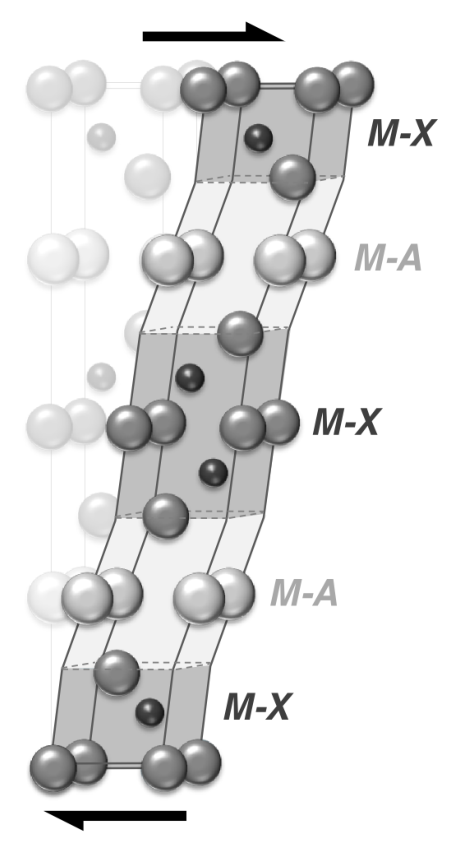
\includegraphics[height=0.3\textheight]{slab_model}
\caption[Hetergeneous strain in a sheared MAX phase unit cell.]{Schematic of non-uniform elastic deformation in a ``211'' MAX phase showing the regions that might be considered distinct, the M--A and M--X layers.\label{fig:slab_model}}
\end{figure}


\captionsetup{width=\textwidth,font={sf,scriptsize},labelfont=bf}


The overall shear modulus for the whole crystal structure is calculated in the same manner with no restrictions on the atomic positions, all the atoms are allowed to relax fully. Since this relaxed shear is equivalent to a uniform applied stress, an analogy is possible with with calculation of the transverse stiffness of long fibre composite materials, the so called slab model \cite{Hull1996ch4}. The slab model is illustrated in \autoref{fig:slab_model}. The results of the local calculations can be compared with the overall case using the equation:
\begin{equation}
G_{\text{slab}} = \left[ \frac{f_{M\text{--}X}}{G_{M\text{--}X}} + \frac{f_{M\text{--}A}}{G_{M\text{--}A}} \right]^{-1} \label{eqn:slab_model}
\end{equation}
where $G_{\text{slab}}$ is the estimate for the overall shear modulus, $f_i$ is the volume fraction of the region $i$ and $G_i$ is the shear modulus of region $i$. The volume fractions are estimated from the crystal structures of the MAX phases. In particular the fractional coordinate in the $c$ direction of the M1 site in the 211 phases, $z_1$, and the position of the M2 site in the 312 and 413 phases, $z_2$, as shown in \autoref{fig:MAX_unit_cells}, determines the volume fraction of the regions of the unit cell:

\begin{subequations}
\begin{align}
f_{\text{M--A}} &= 
\begin{cases}
1-4z_1 & \qquad \text{for 211 phases} \\
4z_2 & \qquad \text{for 312 and 413 phases}
\end{cases}  \\[1ex]
f_{\text{M--X}} &= 
\begin{cases}
4z_1 & \qquad \text{for 211 phases} \\
1 - 4z_2 & \qquad \text{for 312 and 413 phases}
\end{cases}
\end{align}
\end{subequations}

\section{Results and Discussion}

The moduli of the separate layers are presented in \autoref{fig:Gma_variation} and summarised in \autoref{tab:MAX_DFT_elastic_results}. The M--X layer is stiffer than the M--A layer for all the MAX phases studied here, as expected from the nature of the bonding in the MAX phases as discussed in \autoref{sec:layered_crystals}. There is an overall increase in the stiffness of the M--X layer and an overall decrease in the stiffness of the M--A layer as the electronegativity difference between these layers increases, although the data are scattered around that correlation, presumably as more complex chemical factors operate in addition to electronegativity differences.


The trend is clearer when the ratio of the moduli is considered, as shown in \autoref{fig:ratio_of_Gma_to_Gmx}. The ratio $G_{\text{M--A}}/G_{\text{M--X}}$ varies with the electronegativity difference between the layers, so even where other chemical effects cause the overall bonding to be stronger, the \emph{relative} moduli of the two layers are altered by electrons being drawn from the M--A layer into the M--X layer to varying extents. In the case of A atoms like indium or gallium electrons are easily lost from the M--A layer to the M--X layer, reducing the ratio, while in the case of sulphur occupying the A site there is almost no electronegativity difference between the layers and the ratio is higher.


\begin{figure}
\centering

\begin{subfigure}{0.4\textwidth}
\centering
\captionsetup{font={sf,scriptsize},labelfont=bf}
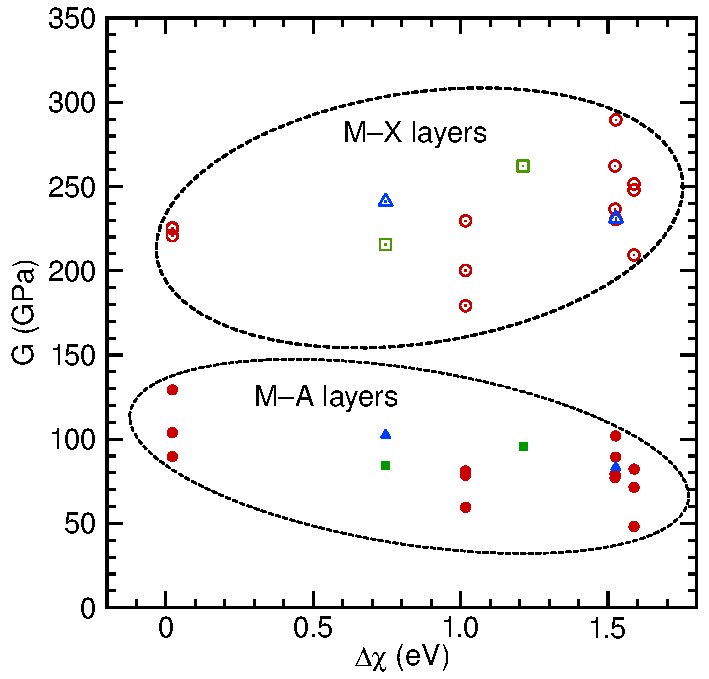
\includegraphics[width=\textwidth]{Gmx_and_Gma_dX_MAX}
\caption{The variation of shear moduli of the M--A and the M--X layers.  \label{fig:Gma_variation}}
\end{subfigure}
~
\begin{subfigure}{0.4\textwidth}
\centering
\captionsetup{font={sf,scriptsize},labelfont=bf}
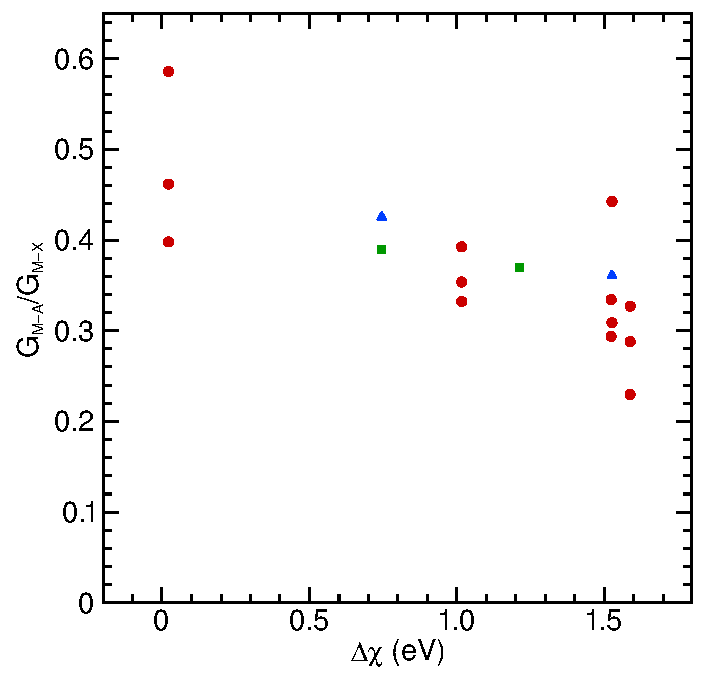
\includegraphics[width=\textwidth]{Gma_Gmx_vs_dX}
\caption{The variation of the ratio of the shear moduli of the M--A and the M--X layers. \label{fig:ratio_of_Gma_to_Gmx}}
\end{subfigure}

\begin{subfigure}{0.4\textwidth}
\centering
\captionsetup{font={sf,scriptsize},labelfont=bf}
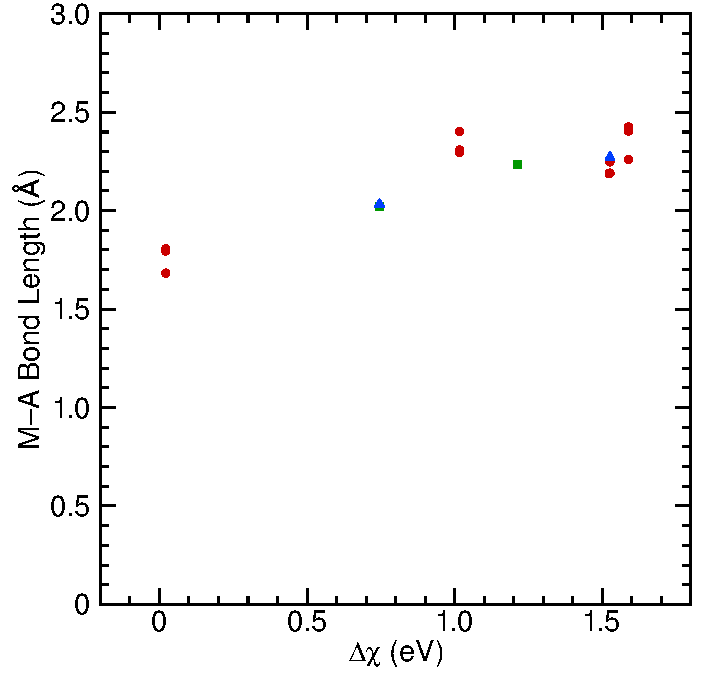
\includegraphics[width=\textwidth]{dma_vs_dX}
\caption{The variation of the M--A bond length. \label{fig:bond_length}}
\end{subfigure}
~
\begin{subfigure}{0.4\textwidth}
\centering
\captionsetup{font={sf,scriptsize},labelfont=bf}
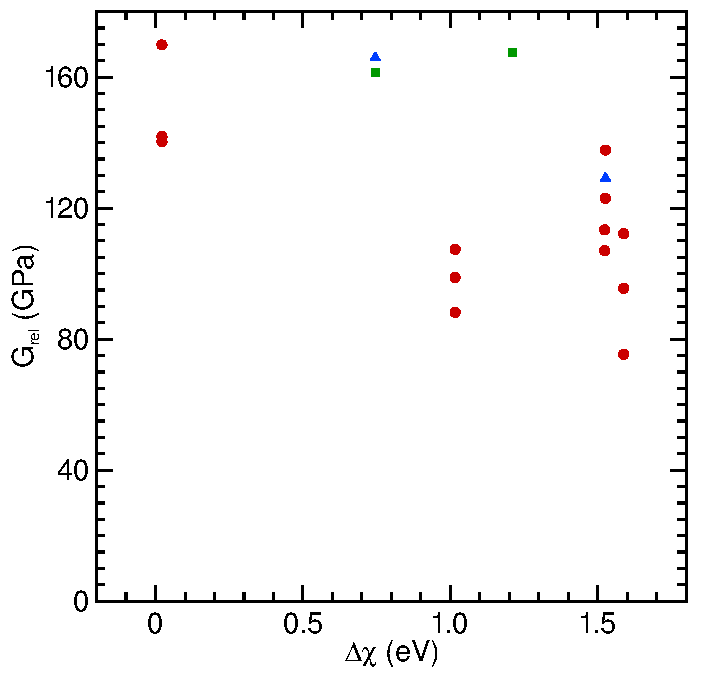
\includegraphics[width=\textwidth]{Grel_vs_dX}
\caption{The variation of the overall shear modulus, $G_{\text{rel}}$. \label{fig:overall_G_vs_dX}}
\end{subfigure}

\begin{subfigure}{\textwidth}
\centering
\captionsetup{width=0.6\textwidth,font={sf,scriptsize},labelfont=bf}
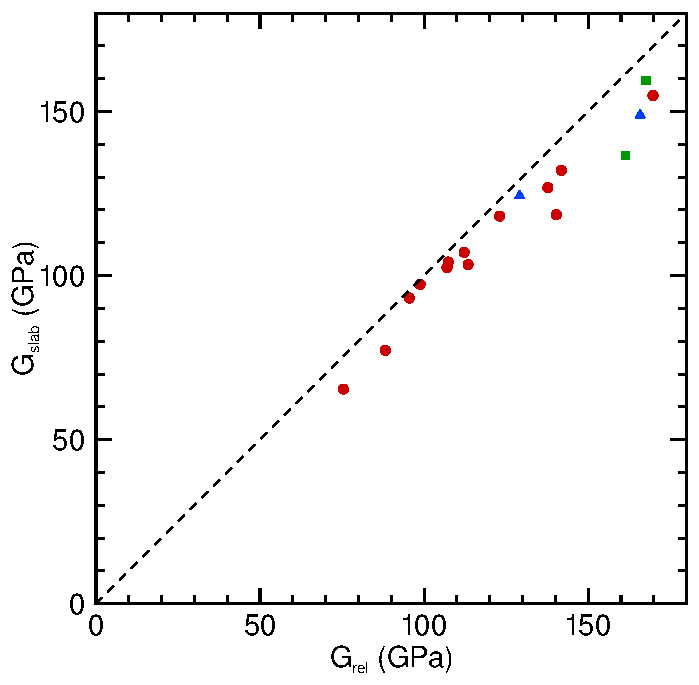
\includegraphics[width=0.4\textwidth]{Gslab_vs_Grel}
\caption{A comparison of the overall shear modulus of the MAX phases, $G_{\text{rel}}$, and the shear modulus calculated from the local shear moduli using the slab model, $G_{\text{slab}}$. The dotted line is $y=x$. \label{fig:Gslab_vs_Grel}}
\end{subfigure}

\caption[The local elastic properties of the MAX phases.]{The results of modelling by DFT the elastic properties of the MAX phases. $\Delta \chi$ is the electronegativity difference between the M--A and M--X layers. Circles, squares and triangles represent 211, 312, and 413 phases respectively.}

\end{figure}

\begin{table}
\centering
\begin{tabular}{|l|c|c|c|c|c|c|}
\hline
Phase \rule[3ex]{0pt}{0pt} &  $G_{\text{rel}}$ &     $G_{\text{M--A}}$ &    $G_{\text{M--X}}$ &  $G_\text{slab}$ &  $G_{\text{M--A}}/G_{\text{M--X}}$ &  $\Delta \chi$ \\
\hline
\ce{Nb2AlC} \rule[3ex]{0pt}{0pt}   &     137.7 &  101.9 &  230.4 &  127.4 &      0.442 &   1.5260 \\
\ce{Nb2GaC}                        &     113.4 &   79.1 &  236.6 &  103.6 &      0.334 &   1.5233 \\
\ce{Nb2In}                         &     112.2 &   82.3 &  251.6 &  105.9 &      0.327 &   1.5880 \\
\ce{Nb2SC}                         &     141.8 &  103.9 &  225.1 &  130.4 &      0.462 &   0.0214 \\
\ce{Nb2SnC}                        &     107.4 &   81.2 &  229.5 &  103.5 &      0.354 &   1.0166 \\
\ce{Ti2AlC}                        &     123.0 &   89.3 &  289.5 &  116.5 &      0.308 &   1.5260 \\
\ce{Ti2GaC}                        &     107.0 &   77.0 &  262.2 &  101.5 &      0.294 &   1.5233 \\
\ce{Ti2InC}                        &      95.5 &   71.4 &  248.0 &   92.1 &      0.288 &   1.5880 \\
\ce{Ti2SC}                         &     169.8 &  129.3 &  220.8 &  154.3 &      0.586 &   0.0214 \\
\ce{Ti2SnC}                        &      98.8 &   78.6 &  200.2 &   97.8 &      0.393 &   1.0166 \\
\ce{Zr2InC}                        &      75.4 &   48.1 &  209.3 &   65.8 &      0.230 &   1.5880 \\
\ce{Zr2SC}                         &     140.3 &   89.7 &  225.4 &  118.1 &      0.398 &   0.0214 \\
\ce{Zr2SnC}                        &      88.2 &   59.5 &  179.1 &   77.1 &      0.332 &   1.0166 \\
\ce{Ti3AlC2}                       &     129.1 &   83.3 &  230.9 &  101.8 &      0.361 &   1.5260 \\
\ce{Ti3SiC2}                       &     165.9 &  102.5 &  241.0 &  144.5 &      0.425 &   0.7453 \\
\ce{Nb4AlC3}                       &     167.6 &   95.8 &  262.2 &  159.5 &      0.365 &   1.2117 \\
\ce{Ti4SiC3} \rule[-1ex]{0pt}{0pt} &     161.4 &   84.3 &  215.6 &  138.1 &      0.391 &   0.7453 \\
\hline
\end{tabular}


\caption[Summary of the elastic properties calculated by density functional theory calculations.]{Summary of the elastic properties calculated by density functional theory calculations.\label{tab:MAX_DFT_elastic_results}}
\end{table}

This change is reflected in the bond lengths in the M--A layers, the bonds getting longer as electronegativity increases. This reflects a weakening of the bonds in the M--A layer as electrons are removed to the M--X layer.




The overall shear modulus was calculated in the same manner and also shows some variation with the electronegativity difference. The overall modulus is calculated by imposing an overall strain on the unit cell and allowing the atomic positions to relax, hence this is termed the relaxed modulus, $G_{\text{rel}}$. There is an overall decrease in the shear modulus of the MAX phases as the electronegativity difference across the structure increases, the contribution of the weakening M--A bond lowering the overall shear modulus more than the strengthening of the M--X bonding raises it.


The slab model was used to compare the local moduli, $G_{\text{M--A}}$ and $G_{\text{M--X}}$,  with the overall modulus, $G_{\text{rel}}$, using \autoref{eqn:slab_model}. The results are plotted in \autoref{fig:Gslab_vs_Grel}. The correlation is very good, showing that the local properties are in agreement with the macroscopic properties.

\captionsetup{font={sf,scriptsize},labelfont=bf}


\section{Conclusions}

The MAX phases have been modelled with density functional theory calculations. The unit cells were optimised and found to be in good agreement with the literature. These unit cells formed the basis of further investigation.

The shear modulus of the M--A and M--X regions of the structure were investigated as well as that of the entire MAX phase structure. The shear modulus was calculated by examining the energy changes for a range of applied shear strains up to \SI{2}{\percent} and fitting to Hooke's law.

The shear moduli of both the M--A layer and the M--X layer varied with the electronegativity difference between them, as the difference increased (M--X becoming more electronegative) the M--A layer became more compliant and the M--X layer became stiffer. In particular the ratio of these moduli was well correlated with the electronegativity difference between the M--X and M--A layers.

The moduli of these regions of the unit cell were combined with the slab model to estimate the overall shear modulus, which matched well with DFT simulations of strains applied to the whole unit cell.





























